\documentclass[12pt]{article}
\usepackage[margin=1in]{geometry} 
\usepackage{amsmath,amsthm,amssymb,amsfonts,bbm}
\usepackage[utf8]{inputenc}
\usepackage[english]{babel}
\usepackage{hyperref}
\usepackage{tikz}
\usetikzlibrary{trees}
\usetikzlibrary{matrix}

\newcommand{\N}{\mathbb{N}}
\newcommand{\Z}{\mathbb{Z}}

\newenvironment{problem}[2][Problem]{\begin{trivlist}
		\item[\hskip \labelsep {\bfseries #1}\hskip \labelsep {\bfseries #2.}]}{\end{trivlist}}
\newenvironment{Lemma}[2][Lemma]{\begin{trivlist}
		\item[\hskip \labelsep {\bfseries #1}\hskip \labelsep {\bfseries #2.}]}{\end{trivlist}}
%If you want to title your bold things something different just make another thing exactly like this but replace "problem" with the name of the thing you want, like theorem or lemma or whatever
\newtheorem{theorem}{Theorem}[section]
\newtheorem{corollary}{Corollary}[theorem]
\newtheorem{lemma}{Lemma}
\begin{document}

	
	\title{The Binomial No-Arbitrage Pricing Model}
	\author{Peiliang Guo}
	\maketitle
	\begin{problem}{1}
	\end{problem}
	If $X_0=0$, 
	$X_1=\Delta_0(S_1-(1+r)S_0)$
	i.e.\begin{align*}
	X_1(H) &= \Delta_0S_0(u-1-r)\\
	X_1(T) &= \Delta_0S_0(d-1-r)
	\end{align*}
	Since we need to have $0<d<1+r<u$, if $X_1$ takes positive value with positive probability (it has to be one of the case), then it will have to be negative in the other.
	\begin{problem}{2}\end{problem}
	From$X_1 = \Delta_0S_1+\Gamma_0(S_1-5)^+-\frac{5}{4}(4\Delta_0+1.20\Gamma_0)$, we know that
	\begin{align*}X_1(H) &= 8\Delta_0+3\Gamma_0-5\Delta_0-1.5\Gamma_0=3\Delta_0+1.5\Gamma_0\\
	X_1(T) &= 2\Delta_0-5\Delta_0-1.5\Gamma_0=-3\Delta_0-1.5\Gamma_0
	\end{align*}
	i.e. $X_1(H)=-X_1(T)$. Therefore, if we have the value of $X_1$ being strictly positive in one case, it will have to be strictly negative in the other.
	\begin{problem}{3}\end{problem}
	\begin{align*}V_0 =& \frac{1}{1+r}[\tilde{p}V_1(H)+\tilde{q}V_1(T)]\\
				=&\frac{1}{1+r}[\tilde{p}S_1(H)+\tilde{q}S_1(T)]\\
				=&S_0\end{align*}
	The last equality comes from the definition of $\tilde{q}$
	\begin{problem}{4}\end{problem}
	\begin{align*}
	X_{n+1}(\omega_1...\omega_nT)=\Delta_n(\omega_1...\omega_n)dS_n(\omega_1...\omega_n)+(1+r)\left(X_n(\omega_1...\omega_n)-\Delta_n(\omega_1...\omega_n)S_n(\omega_1...\omega_n)\right)
	\end{align*}
	Suppress $\omega_1...\omega_n$ and write equation as 
	$$X_{n+1}(T) = \Delta_ndS_n+(1+r)(X_n-\Delta_nS_n)$$
	Also, we have $$\Delta_n=\frac{V_{n+1}(H)-V_{n+1}(T)}{S_{n+1}(H)-S_{n+1}(T)}=\frac{V_{n+1}(H)-V_{n+1}(T)}{(u-d)S_n}$$
	Substituting equation above and $X_n=V_n$ into previous equation to get 
	\begin{align*}X_{n+1}(T) =& \frac{d(V_{n+1}(H)-V_{n+1}(T)}{u-d} +(1+r)\left(X_n-\frac{V_{n+1}(H)-V_{n+1}(T)}{u-d}\right)\\
	=&(1+r)V_n - \frac{1+r-d}{u-d}(V_{n+1}(H)-V_{n+1}(T))\\
	=&\tilde{p}V_{n+1}(H)+\tilde{q}V_{n+1}(T)-\tilde{p}V_{n+1}(H)+\tilde{p}V_{n+1}(T)\\
	=&\tilde{p}V_{n+1}(T)+\tilde{q}V_{n+1}(T)\\
	=&V_{n+1}(T)
	\end{align*}
	\begin{problem}{5}\end{problem}
	$$\Delta_1(H)=\frac{V_2(HH)-V_2(HT)}{S_2(HH)-S_2(HT)}=\frac{3.2-2.4}{16-4}=\frac{1}{15}$$
	This costs $8/15$ dollars and leaves $2.24-8/15 = 1.706667$ dollars to invest in the money market. At time two, she will have $2.13333$ in the money market. If the stock goes up to 16, the stocks will worth $1.066667$, so she will end up with $2.13333+1.066667 = 3.2 = V_2(HH)$ in her portfolio. If the stock goes down to 4, the portfolio value will be $2.13333+0.26667 = 2.4 = V_2(HT)$.\\
	Now assume if the stock goes down in the second period.
	$$\Delta_2(HT) = \frac{V_3(HTH) - V_3(HTT)}{S_3(HTH) -S_3(HTT)} = \frac{0-6}{8-2}=-1$$
	Cost of stock at time 2: $-4$\\
	Investment in the money market: $6.4$\\
	Amount in the money market at time 3: $8$\\
	Stock value if stock goes up in period 3: $-8$ $\Rightarrow  8-8 = 0=V_3(HTH)$\\
	Stock value if stock goes down in period 3: $-2$ $\Rightarrow  8-2 = 6=V_3(HTT) $\\
	\begin{problem}{6}\end{problem}
	$$\Delta_0 = \frac{V_1(H)-V_1(T)}{S_1(H) - S_1(T)}=\frac{3-0}{8-2} = 0.5$$
	Therefore, to gain risk-free on the capital, the trader has to short $0.5$ unit of stock and invest $\Delta_0S_0 = 2$ dollars in the money market, so that at $t_1$\\
	If the stock goes up to 8, the investor has
	$$(8-5)^+-0.5(8)+2(1.25) = 3-4+2.5 = 1.5$$
	If the stock goes down to 2, the investor has
	$$(2-5)^+-0.5(2)+2(1.25) = 0-1+2.5 = 1.5$$
	\begin{problem}{7}\end{problem}
	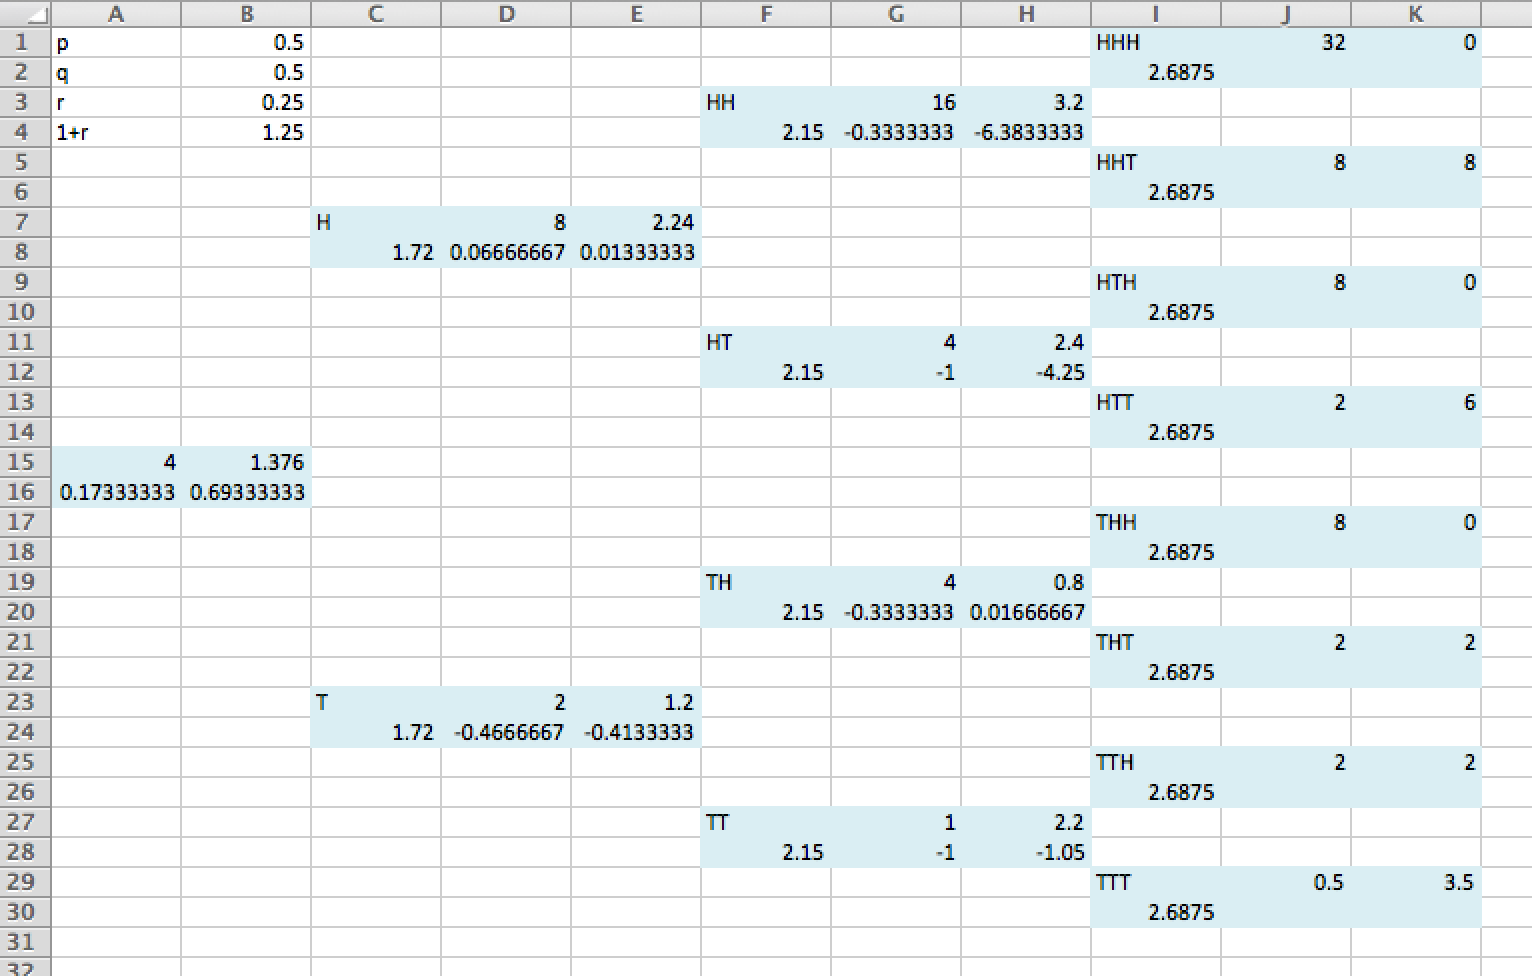
\includegraphics[scale=0.6]{Ex1_7.png}
	\begin{problem}{8}\end{problem}
	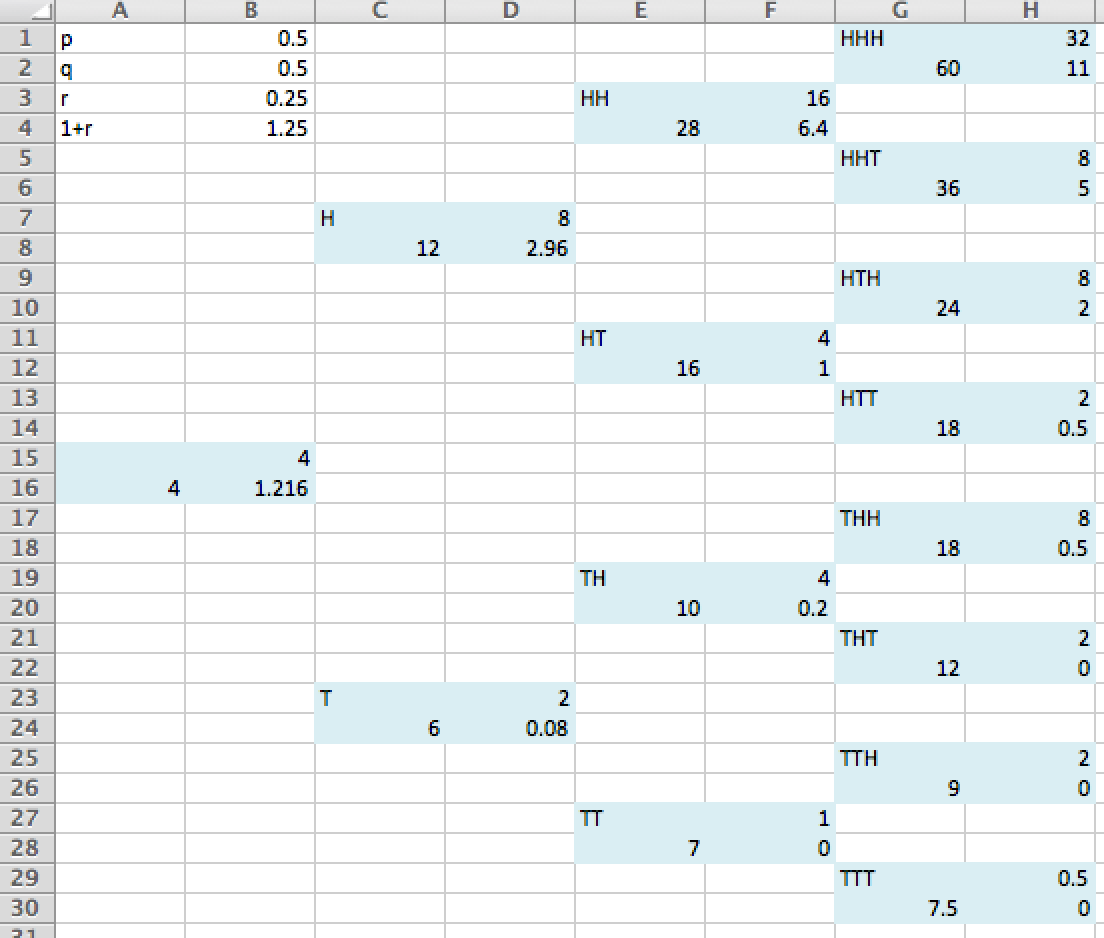
\includegraphics[scale=0.6]{Ex1_8.png}\\
	\begin{align*}
	v_3(32,60) &= (\frac{1}{4}60-4)^+=11\\
	v_3(8,36) &= (\frac{1}{4}36-4)^+=5\\
	v_3(8,24) &= (\frac{1}{4}24-4)^+=2\\
	v_3(2,18) &= (\frac{1}{4}18-4)^+=0.5\\
	v_3(8,18) &= (\frac{1}{4}18-4)^+=0.5\\
	v_3(2,12) &= (\frac{1}{4}12-4)^+=0\\
	v_3(2,9) &= (\frac{1}{4}9-4)^+=0\\
	v_3(0.5,7.5) &= (\frac{1}{4}7.5-4)^+=0\\
	v_2(16,28) &= \frac{1}{1+r}[\tilde{p}v_3(32,60)+\tilde{q}v_3(8,36)] = 6.4\\
	v_2(4,16) &= \frac{1}{1+r}[\tilde{p}v_3(8,24)+\tilde{q}v_3(2,18)] = 1\\
	v_2(4,10) &= \frac{1}{1+r}[\tilde{p}v_3(8,18)+\tilde{q}v_3(2,12)] = 0.2\\
	v_2(1,7) &= \frac{1}{1+r}[\tilde{p}v_3(2,9)+\tilde{q}v_3(0.5,7.5)] = 0\\
	v_1(8,12) &= \frac{1}{1+r}[\tilde{p}v_2(16,28)+\tilde{q}v_2(4,16)] = 2.96\\
	v_1(2,6) &= \frac{1}{1+r}[\tilde{p}v_2(4,10)+\tilde{q}v_2(1,7)] = 0.08\\
	v_0(4,4) &= \frac{1}{1+r}[\tilde{p}v_1(8,12)+\tilde{q}v_1(2,6)] = 1.216
	\end{align*}
	\begin{problem}{9}\end{problem}
	(i) At each state in time $n$, define 
	$$\tilde{p}(\omega_1...\omega_n) = \frac{1+r(\omega_1...\omega_n)-d(\omega_1...\omega_n)}{u(\omega_1...\omega_n)-d(\omega_1...\omega_n)}\text{ and } \tilde{q}(\omega_1...\omega_n) = 1-\tilde{p}(\omega_1...\omega_n)$$
	Then the price of the derivative paying $V_N$ at time $N$ can be computed recursively, backward in time, by the formula
	$$V_n(\omega_1...\omega_n)=\frac{1}{1+r(\omega_1...\omega_n)}[\tilde{p}(\omega_1...\omega_n)V_{n+1}(\omega_1...\omega_nH)+\tilde{q}(\omega_1...\omega_n)V_{n+1}(\omega_1...\omega_nT)]$$
	(ii) $$\Delta_n(\omega_1...\omega_n)= \frac{V_{n+1}(\omega_1...\omega_nH)-V_{n+1}(\omega_1...\omega_nT)}{S_{n+1}(\omega_1...\omega_nH)-S_{n+1}(\omega_1...\omega_nT)}$$
	(iii) First notice that the states are path-independent, so the tree is recombining.
	Also, since $r=0$, we have $$\tilde{p}(\omega_1...\omega_n) = \frac{1-d(\omega_1...\omega_n)}{u(\omega_1...\omega_n)-d(\omega_1...\omega_n)} = \frac{1}{2}$$
	i.e. $\tilde{p}$ is constant at 0.5, thus $V_n(\omega_1...\omega_n) = \frac{V_{n+1}(\omega_1...\omega_nH)+V_{n+1}(\omega_1...\omega_nT)}{2}$. Therefore, 
	\begin{align*}V_0 =& \sum_{i=0}^5{5 \choose i}2^{-5}(20i - 50)^+ = 2^{-5}(50+5(30)+10(10))=9.375\end{align*}
	 \end{document}

	